%--------------------------------------------------------%
%	TITLE
%--------------------------------------------------------%

\chapter[Mean flow direction modulates non-Fickian transport in a heterogeneous alluvial aquifer-aquitard system]{Mean flow direction modulates non-Fickian transport in a heterogeneous alluvial aquifer-aquitard system.\footnote[1]{This chapter will be submitted to \textit{Water Resources Research}: Pauloo, R. A., Fogg, G. E., Guo, Z. \& Henri, C. V. ``Mean flow direction modulates non-Fickian transport in a heterogeneous alluvial aquifer-aquitard system''.}}

%--------------------------------------------------------%
%	ABSRACT
%--------------------------------------------------------%
\section{Abstract}

\noindent Regional-scale groundwater quality degradation from nonpoint source pollution threatens the long-term %water quality 
sustainability of major alluvial aquifer-aquitard systems worldwide. Upscaled transport models can efficiently model regional nonpoint source transport, but fail to accurately characterize non-Fickian (anomalous) transport caused by transience in the mean flow direction. %Owing to the large spatial and temporal scale of nonpoint source pollution, the lack of field data, and uncertainty in geologic heterogeneity, upscaled contaminant transport models are needed. These upscaled models must accurately characterize non-Fickian (anomalous) transport caused by transience in the mean flow direction. 
In this study we demonstrate that hydrogeologic factors explain this failure. Specifically, vertical anisotropy in K and seasonal pumping and recharge in typical alluvial aquifer systems can %cause vertical hydraulic gradient values to exceed horizontal hydraulic gradient values by 10-100 times, 
fundamentally change hydraulic gradients and shift the mean flow direction between mostly horizontal and mostly vertical flow. In order to understand the relationship between large shifts in mean flow direction and transport phenomena, we simulate 3D flow and transport of a conservative solute in a heterogeneous alluvial aquifer under varying mean flow directions representative of typical seasonal hydraulic gradient fluctuations. We examine tailing, plume spreading, and the spatial distribution of final particle positions. Results indicate that alterations to hydraulic gradients which control the mean flow direction can lead to increasingly non-Fickian transport. %At low VHGR (e.g., ambient hydraulic gradient conditions that correspond to a more horizontal flow direction), 
When flow is mostly horizontal, diffusion and slow advection dominant low-K facies slow mass transfer rates out of low-K material, and preferential flow along connected high-K networks cause increased spatial spreading along the mean flow direction. In contrast, %high VHGR (e.g., 
predominantly vertical flow caused by spatially distributed pumping and recharge shifts mass transfer processes in low-K material from diffusion and slow advection dominant to advection dominant, which results in vertically oriented particle trajectories that compactly migrate through high and low K facies alike, and leads to increasingly Fickian transport. Thus, fluctuations in mean flow direction driven by vertical anisotropy of K and seasonal pumping and recharge in a typical alluvial aquifer-aquitard system create oscillating patterns of transport, ranging from persistently non-Fickian to more Fickian. Results %bear importantly on the management and modeling of widespread nonpoint source contamination in alluvial basins worldwide, and 
illustrate the hydrogeologic factors that explain why upscaled transport models fail to capture non-Fickian transience in mean flow direction.

%--------------------------------------------------------%
%	INTRO
%--------------------------------------------------------%
\section{Introduction}

Basin-scale groundwater quality in alluvial aquifer systems is threatened by nonpoint source contaminants including agricultural fertilizers \citep{Burow2008}, pesticides \citep{Burow2008, Burow1998}, nitrates \citep{Harter2012, henri2019stochastic}, and total dissolved solids \citep{Hansen2018, Lindsey2018} on large temporal (e.g., decades to centuries) and spatial scales (e.g., tens to hundreds of kilometers). Thus, regional groundwater quality management models \citep{Fogg2006} are needed that can robustly represent non-Fickian (i.e., anomalous) transport under a range of geologic heterogeneity and transient flow boundary conditions encountered on large temporal and spatial scales. However, modeling regional nonpoint transport remains a challenging task due to %differences between the temporal and spatial scales at which processes are typically measured and modeled \citep{cushman2002primer, bastani2020effects}, and due to 
ubiquitous non-Fickian spreading which is difficult to model at regional scales with existing approaches, especially when the boundary conditions shift from steady state to transient flow \citep{guo2020adaptive, labolle2001role}.

Transport modeling is challenged by non-Fickian transport across pore \citep{kang2014pore, morales2017stochastic}, field \citep{garabedian1991large, le2008non}, and regional scales \citep{sivakumar2005fractal, henri2019stochastic}, and in diverse heterogeneous geologic formations such as alluvial aquifers \citep{weissmann2002dispersion, labolle2001role, guo2019upscaling} and discrete fracture networks \citep{hyman2015influence, edery2016structural}. Non-Fickian transport may be measured by features including nonlinear scaling of the second spatial moment (i.e., the mean squared displacement), early breakthrough, and late-time arrival (i.e., tailing) of solutes \citep{valocchi1985validity, freyberg1986natural, zhang2007predicting, haggerty2000late}. The ubiquity of non-Fickian effects across disciplines and natural systems, and the inherent uncertainty in characterizing the scale and space-time dependencies of anomalous transport in heterogeneous media has led to multiple conceptualizations of how to mathematically model and upscale non-Fickian transport \citep{neuman2009perspective}.

Numerous studies show that anomalous transport in geologic media depends strongly on spatially heterogeneous hydraulic conductivity \citep{gelhar1993stochastic, dagan2005subsurface, de2005dealing}, which gives rise to the velocity field \citep{berkowitz2006modeling}. In many alluvial aquifer-aquitard complexes, variability in the hydraulic conductivity ($K$) of sediments can range over 4-7 orders of magnitude \citep{Fetter2001, fogg2016debates}. The fluvial deposition processes that form alluvial aquifer-aquitard systems over millennia result in correlated fields \citep{galloway2012terrigenous}, with interconnecting, high-K, coarse sand and gravel lenses \citep{fogg1986groundwater} that can percolate in all spatial dimensions \citep{fogg2000connected}, even at substantially low volume fractions, such as 13\% as noted in 3D percolation studies by \citet{harter2005finite}. These high-K preferential flowpaths facilitate anomalous early time arrival, and are embedded within low-K, fine-grained clays and silts, which typically comprise the majority of alluvial aquifer-aquitard volume fractions \citep{galloway2012terrigenous}, and contribute to mass hold back and anomalous late-time solute tailing \citep{labolle2001role, berkowitz2006modeling, haggerty2000late, benson2000application}. Moreover, in typical alluvial heterogeneous material, where the horizontal length scales of K variability are often 2-3 orders of magnitude or more larger than vertical length scales of K variability, \citet{zhang2006nonpoint} found that vertical transport is increasingly Fickian under more anisotropic conditions. %Thus, stochastic hydrofacies models \citep<e.g.>{carle1996transition} which explicitly represent the geologic heterogeneity that gives rise to non-Fickian transport are a powerful tool to understand flow and transport properties of subsurface plumes, and have greatly informed the development of upscaled models \citep<e.g.>{guo2020adaptive}.

The interaction between spatial heterogeneity and hydraulics determines transport processes. However, anomalous transport studies commonly investigate simple hydraulic boundary conditions characterized by a unidirectional gradient \citep{benson2001fractional, edery2014origins, edery2016structural, harvey2000rate, pedretti2014apparent, willmann2008transport, leblanc1991large, julian2001numerical, Zhang1999nonideal, henri2015random}, which is typical of natural, ambient groundwater flow \citep[e.g. a horizontal hydraulic gradient on the order of $10^{-3}$][]{Fetter2001}. Many of these studies hold hydraulic boundary conditions constant in order to investigate how changing the spatial heterogeneity of the domain impacts solute transport. However, because of horizontal stratification of coarse- and fine-grained facies typical of many clastic sedimentary environments and hence significant vertical anisotropy of effective hydraulic conductivity (K), the vertical hydraulic gradients commonly exceed horizontal gradients by a factor of $10^1 - 10^2$ \citep[e.g.][]{fogg1986groundwater, belitz1993numerical}. In even moderately developed groundwater basins, and especially in agriculturally intensive ones, high rates of seasonal pumping and recharge from irrigation can further increase vertical hydraulic gradients \citep{styles1999subsurface, gailey2018using}. Yet, only a few modeling studies investigate non-Fickian transport under such large shifts in regional hydraulic gradient, and these studies tend to emphasize local scale breakthrough measured at extraction wells or control planes. \citet{matheron1980transport} demonstrated in a 2D model with limited spatial heterogeneity that flow parallel to the bedding direction leads to preasymptotic anomalous transport, even at very long timescales because the solute travels along an increasingly non-stationary medium. \citet{henri2019stochastic} demonstrated that well design characteristics (e.g., well depth, pumping rate, and screen length) have a significant impact on the uncertainty of late arrival times generated by heterogeneity. Similarly, \citet{libera2017influence} demonstrated that temporally variable pumping rates strongly affected contaminant breakthrough curves at the pumping well. \citet{guo2019upscaling} investigated anomalous transport arising from the transition from predominately horizontal to vertical flow, and found that internal hydraulic gradients between the high‐ and low‐K materials strongly affect mass transfer between hydrofacies. Furthermore, \citep{guo2020adaptive} showed that an upscaled multirate mass transfer model failed to capture tailing effects when the mean flow direction changed. Thus, prior work suggests that hydraulic boundary condition transience can strongly impact non-Fickian transport yet we still lack an understanding of how shifting hydraulic gradients (as opposed to the unidirectional gradient that most studies explore) may modulate the degree of anomalous transport observed in a heterogeneous aquifer-aquitard complex. 

To the best of our knowledge, no studies have investigated the impact of non-horizontal and non-vertical mean flow direction on non-Fickian transport within a 3D, kilometer-scale, alluvial aquifer-aquitard system. Such a question bears importantly on modeling macroscopic nonpoint source transport in large alluvial groundwater systems, and may shed light on how to build better upscaled transport models that perform well across a range of transient hydraulic gradient conditions.

In this study, we simulate groundwater flow and random walk particle tracking in a detailed hydrofacies model of a typical alluvial aquifer-aquitard complex (with high vertical anisotropy in K) subject to an increasingly high \textbf{v}ertical to \textbf{h}orizontal hydraulic \textbf{g}radient \textbf{r}atio (VHGR), which is an indicator of the mean flow direction. In other words, if we increase the vertical hydraulic gradients in a system by a factor of 10, 100, or 1000 (e.g., due to natural geologic variation in vertical anisotropy of K, or during the transition from a fallow winter season to a summer growing season characterized by pumping and recharge), does this makes the transport more non-Fickian, and if so, by how much, and why? Changes in anomalous nonpoint source transport are compared between differing steady-state VHGR scenarios which collectively represent snapshots along a transition from predominantly horizontal (low VHGR) to vertical flow (high VHGR). We examine tailing, spatial variance of the nonpoint source plume, and the spatial distribution of final particle position to quantify and explain differences in non-Fickian spreading. Results are discussed in the context of the transition from advection to diffusion dominant systems, and related to the hydrogeology of the study site. We explore how our findings support a conceptualization of regional scale nonpoint source contaminant migration characterized by oscillating patterns of non-Fickian transport, and how this perspective might inform the development of upscaled regional groundwater quality management models \citep{Fogg2006}.




%--------------------------------------------------------%
%	METHODS
%--------------------------------------------------------%
\section{Methods}

First, a heterogeneous, hydrofacies-based geostatistical model of the Kings River alluvial fan in California's Central Valley was developed. Next, four VHGR scenarios of increasingly vertical groundwater flow were simulated, and used to solve the particle transport of a conservative solute. Lastly, the resulting 3D Lagrangian particle trajectories were analyzed in terms of their tailing, second spatial moment, and spatial distribution of final particle position. 

%
%---------------- Hydrofacies model  ------------------%
%
\subsection{Heterogeneous hydrofacies model and study site}
\label{ss_2_1}

The three‐dimensional, spatially-correlated hydraulic conductivity domain (Figure \ref{fig:model}) was simulated with Transition Probability Geostatistical Software (T-PROGS), which uses the transition probability approach described by \citet{carle1996transition, carle1997modeling, carle1999tprogs}. Details of the facies model are provided in \citet{weissmann1999three, weissmann1999multi, weissmann2002glacially, weissmann2004influence}, and a brief summary is provided here.

A subsection of the Central Valley aquifer (California, USA) in the Kings River fan, was chosen as a study site representative of a typical alluvial aquifer for its high vertical anisotropy ($K_h/K_v =$ 238), and its validated performance in simulating both flow (hydraulic head) and transport (groundwater age distribution) \citep{weissmann2002dispersion}. The hydrofacies model was conditioned by analyzing more than 40 000 surface and shallow subsurface ($<$ 2 $m$) features (e.g., borings, excavations, road cuts, and natural exposures) \citep{huntington1981soil}, approximately 150 $m$ of core and geophysical logs \citep{burow1997hydrogeologic}, approximately 1,000 $m$ of continuous core \citep{harter2005deep}, and numerous drillers' logs from water wells in the study area \citep{weissmann1999multi}. These analyses defined a conceptual geologic model and the T-PROGS model parameters. 


% F:\Box Sync\Research\Post QE Research\DISSERTATION\02_ade\code\00_interpolate_paths_extract_trajectories.R
% creates: C:/Users/rpauloo/Documents/GitHub/kings-river-fan-tprogs/code/rw3d//2019_11_20_100s_10kp/dat/part_traj_paraview_00_03.csv
% which is read into Paraview, and edited in Illustrator in C:\Users\rpauloo\Documents\GitHub\kings-river-fan-tprogs\paraview
% Paraview: krf_plus_part_traj_FINAL_00_03.pvsm
% AI: krf_part_traj_00_03.ai
% PNG: krf_part_traj_00_03-01.png
% 01_mm\ai\study_site_water_budget.ai
% numbers come from archived (commented out Table 5)
\begin{figure}[H]
	\centering
	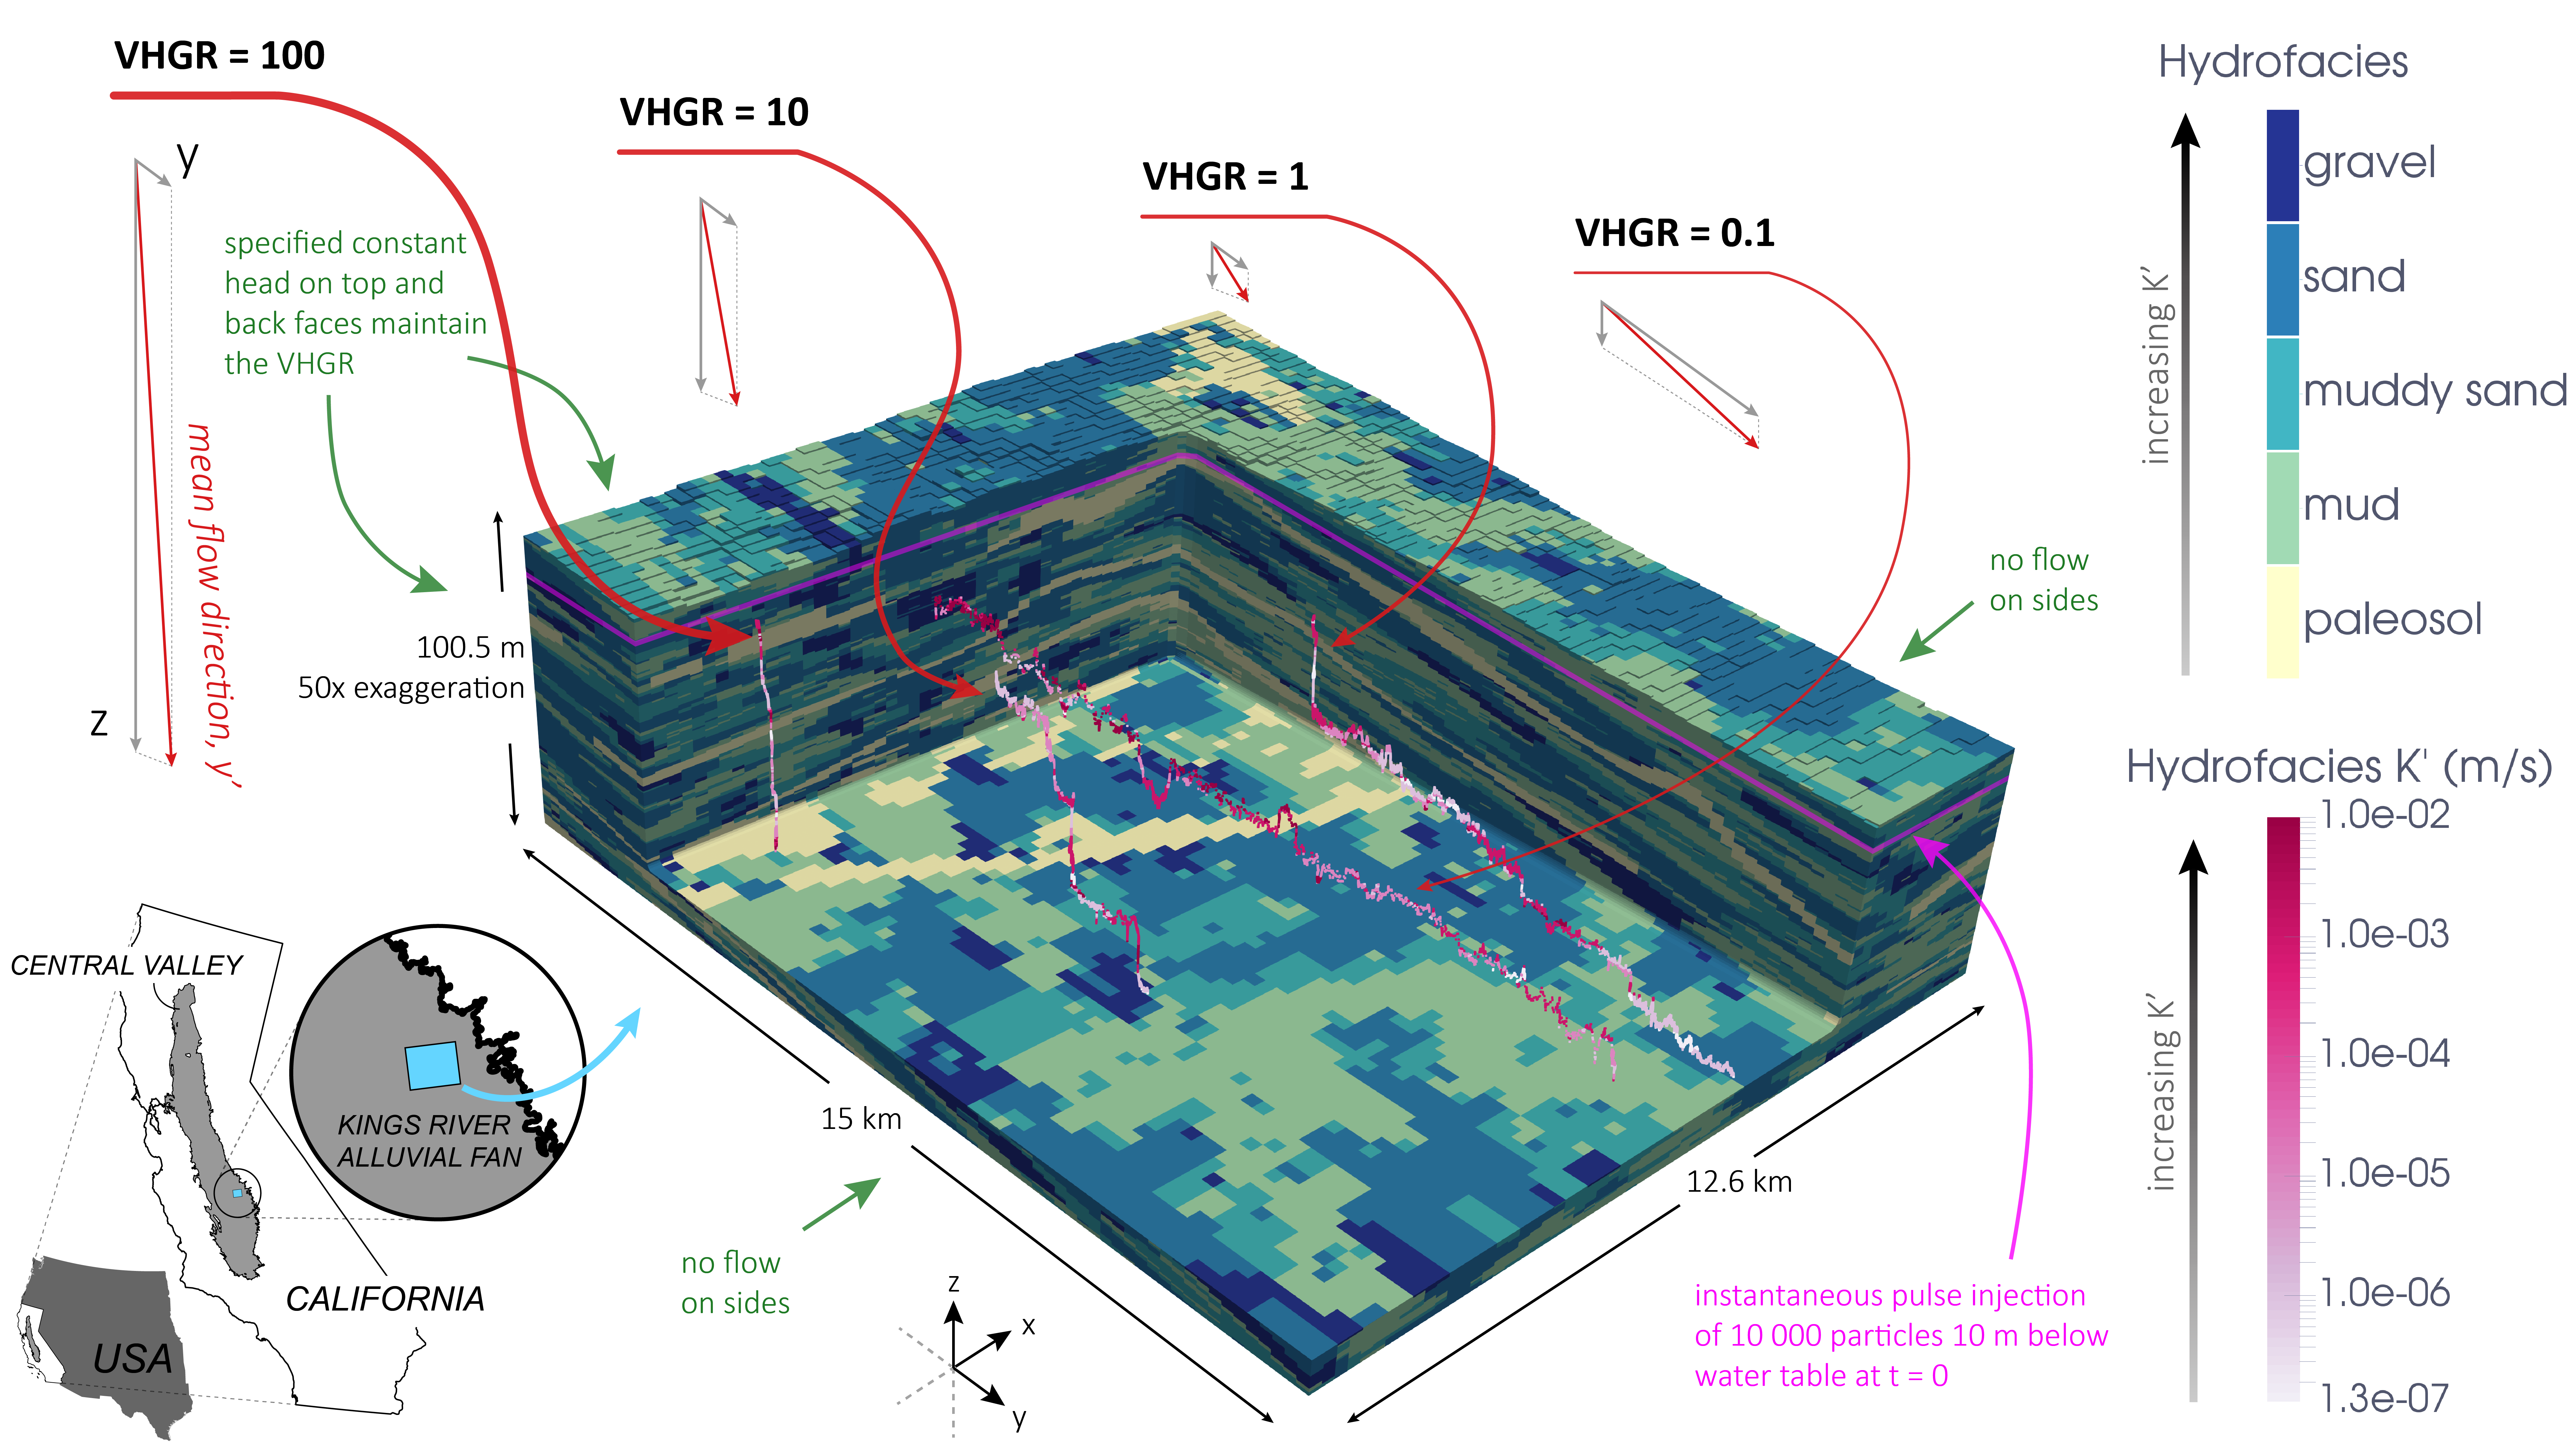
\includegraphics[width=\textwidth]{ch4_figs/krf_part_traj_00_03-01.png}
	\caption{The Kings River alluvial fan hydrofacies model in California's Central Valley (USA) with a section cut away to reveal the geologic heterogeneity and four representative particle trajectories from the four VHGR scenarios in this study (section \ref{ss_2_3}). The location of the instantaneous nonpoint source term (10 000 particles, 10 $m$ below the water table) is represented by a horizontal pink line. Particle trajectories are increasingly horizontal and non-Fickian with decreasing VHGR. Note that the vectors representing flow in $z$, $y$, (and their geometric sum in the mean flow direction, $y'$) are illustrative, and not drawn to scale.}
	\label{fig:model}
\end{figure}


The Kings River alluvial fan is composed of four sequences created during Pleistocene glacial cycles and a fifth basal depositional unit prior to major glaciation events, each separated by laterally-extensive paleosols that formed during inter-glacial periods of pedogenesis \citep{weissmann2002glacially}, which, owing to their relatively low hydraulic conductivity, act as aquitards. Notably, one unit represents a incised valley fill of coarse-grained sediment in the back-to-front $y$ direction of the domain, created by downcutting rivers during high ice-stages (low sea-level) then filled with glacial outwash as glaciers retreated and sea-level rose. Key parameters derived from these analyses that constrained the T-PROGS model include the hydrofacies proportions, mean lengths in $xyz$, and the embedded transition probabilities in $xyz$, which reflect the cross-correlation between facies and thus the probability that one facies contacts another in a given direction \citep{carle1996transition}. Next, Markov chain models corresponding to each unit were developed and combined to represent the highly heterogeneous stratigraphy: overlapping alluvial fans, interspersed with laterally-extensive paleosols, and a cross-cutting incised valley fill. \citet{weissmann2004influence} provides a detailed overview of the development and combination of these models into a single conductivity field. 

The model dimensions in $xyz$ are 12.6 $km$ x 15 $km$ x 100.5 $m$, with discretization $\Delta x = \Delta y = $ 200 $m$, and $\Delta z =$ 0.5 $m$. Spatially variable $K$ estimated from pumping tests, slug tests, core measurements, and literature values for similar lithologies \citep{burow1999evaluation, weissmann1999three} were assigned to each of the model cells by their simulated hydrofacies, which include gravel, sand, sandy mud, muddy sand, and paleosols (Table \ref{tab:model_l_k_pe}).


% F:\Box Sync\Research\Post QE Research\DISSERTATION\02_ade\code\tables.R
% object is called `d`
\bgroup
\begin{table}[ht]
\centering
%\small\addtolength{\tabcolsep}{-5pt}
\resizebox{\textwidth}{!}{%
\begin{tabular}{lrrrlllll}
\hline
Hydrofacies & $l_x (m)$ & $l_y (m)$ & $l_z (m)$ & $K (m/s)$ & $P_e^{100}$ & $P_e^{10}$ & $P_e^{1}$ & $P_e^{0.1}$\\

\hline

gravel & 200 & 650 & 1.5 & 1.0E-02 & 2.05E+09 & 2.05E+08 & 2.05E+07 & 2.05E+06\\
sand & 625 & 1500 & 3.3 & 1.0E-03 & 5.13E+08 & 5.13E+07 & 5.13E+06 & 5.13E+05\\
muddy sand & 400 & 800 & 1.4 & 1.0E-05 & 2.90E+06 & 2.90E+05 & 2.90E+04 & 2.90E+03\\
mud & NA & NA & 1.0 & 1.0E-06 & 289.86 & 28.99& 2.9 & 0.29 \\
paleosol & 800 & 1500 & 1.9 & 1.3E-07 & 71.59 & 7.16 & 0.72 & 0.07\\

\hline
\end{tabular}
} % for \resizebox
\caption{Hyrdofacies properties including mean lengths $l$ in $xyz$ directions (strike, dip, and vertical in Figure \ref{fig:model}), hydraulic conductivity $K$ ($m/s$), and average Peclet number across the VHGR scenarios.}
\label{tab:model_l_k_pe}
\end{table}

\egroup

We only use one realization of the hydrofacies model (Figure \ref{fig:model}) because previous studies demonstrate that the statistics of particle paths, and hence non-Fickian transport behavior does not appreciably differ between realizations due to good connectivity of aquifer facies \citep{guo2019upscaling, weissmann2002dispersion}.


%
%---------------- Groundwater flow simulation  ------------------%
%
\subsection{Groundwater flow and transport simulation}
\label{ss_2_2}

Steady state, groundwater flow in the geostatistical model grid (Section \ref{ss_2_1}) is simulated in MODFLOW \citep{harbaugh2000modflow, mcdonald1988modflow}. The 3D groundwater flow equation used to compute long-term, average confined flow is:   


\begin{equation}
    \frac{\partial{}}{\partial{x}}(K_{xx} \frac{\partial{h}}{\partial{x}}) +
    \frac{\partial{}}{\partial{y}}(K_{yy} \frac{\partial{h}}{\partial{y}}) +
    \frac{\partial{}}{\partial{z}}(K_{zz} \frac{\partial{h}}{\partial{z}}) +
    W = S_s \frac{\partial{h}}{\partial{t}}
\label{eq:gwflow}
\end{equation}

where $K_{xx}$, $K_{yy}$, and $K_{zz}$ [$LT^{-1}$] are the hydraulic conductivities along the $x$, $y$, and $z$ coordinate axes; $h$ $[L]$ is the potentiometric head; $W$ [$T^{-1}$] is the volumetric flux per unit volume of sources ($W >$ 0) or sinks ($W <$ 0); $S_s$ [$L^{-1}$] is the specific storage; and $t$ $[T]$ is time. 

The water table is represented on the top of the domain with a constant head boundary condition, which is the same across all scenarios. Vertical flow out of the bottom of the model and into deeper groundwater, due to a combination of pumping at depth and recharge from above, is represented by another constant head boundary condition on the bottom of the domain, and is altered depending on the VHGR scenario in question (discussed in section \ref{ss_2_3}). Two more constant head boundary conditions on the front and back faces of the model maintain an ambient regional horizontal groundwater flow gradient of 0.001 along the $y$ direction (Figure \ref{fig:model})of the model. Head values are spatially distributed across all active faces such that the mean flow direction is uniform across the entire domain (SI Appendix Figure \ref{ap_c_heads_vhgr}). No flow boundaries are specified along the right and left faces of the domain (along the $x$ direction). 


%Particle tracking transport simulation

Solute transport is simulated by the random‐walk particle tracking method \citep{labolle1998diffusion, labolle2000diffusion} applied in the code RW3D \citep{fernandez2005differences, henri2014toward, henri2015random, salamon2006modeling} that solves the advection-dispersion equation: 

\begin{equation}
    \theta \frac{\partial{c}}{\partial{t}} = \nabla \cdot (\theta D \nabla c) - \nabla \cdot (qc)
\label{eq:ade}
\end{equation}

%\begin{equation}
%    D = (\alpha_T |q| + D^*) \delta + (\alpha_L - \alpha_T)qq^t / |q|
%\label{eq:d}
%\end{equation}

where $c$ is the concentration of the dissolved solute [$ML^{-3}$], $\theta$ is the effective porosity [$-$], and $\textbf{D}$ is the dispersion tensor, defined as $\textbf{D} = (\alpha_T |\textbf{q}| + D^*) \textbf{I} + (\alpha_L - \alpha_T) \textbf{qq}^t / |\textbf{q}|$, where $D^*$ is the molecular diffusion coefficient [$L^2 T^{-1}$], $\alpha_L$ and $\alpha_T$ are the longitudinal and transverse dispersivities [$L$], $\textbf{I}$ is the Dirac delta function, and $|\textbf{q}|$ is the magnitude of the velocity vector [$LT^{-1}$].

The source term is a discrete, instantaneous pulse injection of 10 000 particles at 10 $m$ below the water table (Figure \ref{fig:model}). To simulate the spatial variability of contaminant mass arrival at the water table, flux-weighted injection is used to initialize particle motion. Simulations are run for a sufficient number of time steps such that all particles exit the domain (SI Appendix Table \ref{ap_c_rw3d_params}), and that the mean Lagrangian hydrofacies proportions (i.e., the proportion of particles in each hydrofacies) converge on the actual hydrofacies proportions over time (SI Appendix Figure \ref{ap_c_heads_vhgr}). The Lagrangian particle tracking methods used in this study can be very computationally intensive, especially for the case of a regional-scale nonpoint source term, where the size of the domain (and hence the number of particles used to sample it) is large. Adding multiple injections of particles was computationally unrealistic, and moreover, under steady state flow, a continuous source injection and instantaneous pulse injection yield similar results. %(this is not the case for a transient flow simulation, which we do not investigate). 

\citet{labolle2001role} demonstrated for a similar hydrofacies-based domain that solute transport results were insensitive to local-scale $\alpha$, which was insignificant compared to the dispersion caused by the hydrofacies-scale heterogeneity of the conductivity domain. Moreover, \citet{weissmann2002dispersion} investigated sensitivity analyses with $\alpha_L$ and $\alpha_T =$ 0.1 $m$ and $=$ 0.01 $m$ in the same Kings River Fan domain that we use in this study, and found that between geostatistical realizations, the simulation results did not differ appreciably in terms of the overall transport. Thus, we set longitudinal, transverse horizontal, and transverse vertical dispersivities to 0.01 times the cell discretization, $\alpha_L = \alpha_{TH} = $ 2.0 $m$, and $\alpha_{TV} = $ 0.005 $m$. These local-scale dispersivities were maintained across the VHGR scenarios in order to ensure comparability. We assume a conservative (non-reactive, non-sorbing) solute and set the molecular diffusion coefficient $D^*$ = 6.9E-10 $m^2/s$, based on \citet{weissmann2002dispersion}. 

% $D^* = D_d / \tau^2$ \citep{Fetter2001}, where $D_d$ is an average diffusion coefficient for common ions, 2.0E-9 $m^2/s$, \citep{domenico1998physical} and $\tau$ is an average tortuosity (arc to chord ratio) of 1.7, according to



%---------------- hydraulic gradient scenarios  ------------------%
\subsection{Hydraulic gradient scenarios}
\label{ss_2_3}

The aim of this study is to investigate the influence of mean flow direction on non-Fickian transport, thus we compare systems under different \textbf{v}ertical to \textbf{h}orizontal \textbf{g}radient \textbf{r}atio (\textbf{VHGR}):

\begin{equation}
    VHGR = i_v / i_h
\label{eq:vhgr}
\end{equation}

where $i_v$ is the vertical gradient $\partial{h}/\partial{z}$, and $i_h$ is the horizontal gradient $\partial{h}/\partial{y}$ (Figure \ref{fig:model}). Increasing VHGR corresponds to increasingly vertical flow. Four scenarios are simulated, in which VHGR is varied over four orders of magnitude by fixing $i_h$ = 0.001 (representing ambient horizontal groundwater flow from mountain front recharge), and adjusting $i_v$:

\begin{itemize}
    \item VHGR = 0.1 ($i_v =$ 0.0001): primarily horizontal flow with minimal recharge
    \item VHGR = 1 ($i_v =$ 0.001): equal horizontal and vertical gradients  
    \item VHGR = 10 ($i_v =$ 0.01): substantial component of vertical groundwater flow
    \item VHGR = 100 ($i_v =$ 0.1): dominantly vertical flow 
\end{itemize}


Within-facies heterogeneity (e.g., stratification of coarse and fine facies) can create strong regional vertical anisotropy values on the order of 100:1 or larger \citep{freeze1979groundwater}. In our study site, permeameter tests indicate the ratio between regional-scale effective $K_h$ and $K_v$ is 238, which tends to produce natural values of VHGR $>$ 1 in such systems \citep[e.g.][]{fogg1986groundwater}. 

Groundwater development by pumping can further increase VHGR, and the augmentation of recharge due to irrigation can still further increase it. For example, values of $i_v$ in portions of the Central Valley can vary from order $10^{-3}$ in winter (non-pumping season) to $10^{-1}$ in summer (pumping season). Hence, taken independently, the four steady state VHGR flow fields represent stages along a transition from ambient, primarily horizontal groundwater flow to predominantly vertical flow induced by natrual anisotropy in K and pumping and recharge, and permit an investigation of long-term plume evolution across these different hydraulic gradient conditions. 


Across each VHGR, the Peclet number, $P_e$ (i.e., the ratio of the characteristic time scales of advection to diffusion) was calculated for each hydrofacies (Table \ref{tab:model_l_k_pe}).

\begin{equation}
    P_e = K i l \: / \: D^* \theta
\label{eq:pe}
\end{equation}

where $i$ is the vertical hydraulic gradient of the VHGR scenario and $D^* =$ 6.9E-10 $m^2/s$ \citep{weissmann2004influence, weissmann2002modeling}, and $\theta$ is the hydrofacies porosity. Due to the influence of vertical gradients, $P_e$ of gravel, sand, and muddy sand were calculated using mean horizontal length scales ($l_x, \: l_y$), whereas the $P_e$ of mud and paleosol were calculated using vertical length scales ($l_z$). For gravel, sand, and muddy sand, $\theta =$ 0.3, and for mud and paleosol, $\theta =$ 0.5. Mud was used as a background category, thus its lateral mean lengths ($l_x$ and $l_y$) were already determined in the process of Markov chain modeling of the transition probability \citep{weissmann1999three}.


Generally, system-wide $P_e > 1$ is considered advection dominant, $P_e < 1$ indicates diffusion dominance, and slow advection (which may resemble a more diffusion-like process) may occur at relatively small $P_e$ less than 1 \citep{guswa2000slow}. In heterogeneous aquifer-aquitard systems, which vary in terms of the hydraulic conductivity field, porosity, and hydraulic gradient, $P_e$ varies spatially. Importantly, the $P_e$ of low-K mud and paleosol hydrofacies in this study can transition between advection and diffusion dominance due to changes in flow rates in these hydrofacies caused by different VHGR, with consequences for macroscopic transport behavior. 






%
%---------------- Metrics of non-Fickian transport  ------------------%
%
\subsection{Metrics of non-Fickian transport}
\label{ss_2_5}

In order to compare the impact of various VHGR scenarios on anomalous transport, we measure tailing by fitting a tempered fractional advection-dispersion equation (TFADE) to breakthrough curves and comparing the tempering parameter. Tailing is the late-time arrival of solutes at a control plane, and indicates mass holdback in fines. We also compute the time and space evolution of the mean squared displacement (MSD), or second spatial moment, which measures the variance in plume displacement and represents how ``spread out'' all of the particles are from one another due to mass holdback and preferential flow. Lastly, we investigate the spatial distribution of final particle positions with respect to the site's geologic heterogeneity, which illustrates preferential flow.

Between VHGR scenarios, travel times are re-scaled by $t_c = l_c / \bar{v}$, where $t_c$ is the characteristic travel time to travel the average facies length, and $l_c$ and $\bar{v}$ are the characteristic length and mean velocity along the mean flow direction $y'$ (details provided in SI Appendix Section \ref{s_ap_c_part_rot} and Table \ref{ap_c_tc}). 


%
%---------------- Tailing  ------------------%
%
\subsubsection{Tailing}
\label{ss_tailing}

In order to quantify differences in tailing, a tempered fractional advection-dispersion equation (TFADE) model \citep{meerschaert2008tempered} was fit to breakthrough at a control plane along the bottom face of the model:

\begin{equation}
\label{eq:tfade}
    \frac{\partial C(y', t)}{\partial t}+\beta e^{-\lambda t} \frac{\partial^{\gamma}\left[e^{\lambda t} C(y', t)\right]}{\partial t^{\gamma}}-\beta \lambda^{\gamma} C(y', t)=-V_{L} \frac{\partial C(y', t)}{\partial y'}+D_{L} \frac{\partial^{2} C(y', t)}{\partial y'^{2}}
\end{equation}

where $t$ $[T]$ is time; $C$ $[ML^{-3}]$ is the concentration; $y'$ $[L]$ is the position along the longitudinal direction; $V_L$ $[LT^{-1}]$ is the longitudinal velocity; $D_L$ $[L^2T^{-1}]$ is the molecular dispersion coefficient; $\beta$ $[T^{1/ \gamma}]$ is the fractional capacity coefficient, which governs the mobile fraction; $\gamma$ $[-]$ is the time fractional order; $\lambda$ $[T^{-1}]$ is the tempering parameter. Importantly, $\lambda$ represents the probability that the waiting times in the immobile phase transfer from a power‐law to exponential distribution and thus, provides a quantitative measure of tailing: as $\lambda$ approaches infinity, the TFADE reverts to the classic advection-dispersion equation, and a decreasing $\lambda$ indicates longer tailing. 

We are principally interested in tailing along the bottom face, yet, as VHGR decreases, horizontal flow causes more particles to exit the down-gradient face rather than the bottom face. However, a substantial fraction of 10 000 initial particles exit the bottom face in each simulation: 78.0, 74.7, 16.8, 7.7 \% of particles break through the bottom of the domain after 1000 characteristic times in VHGR = 100, 10, 1, and 0.1 respectively. Thus, to ensure the comparability of breakthrough, we assumed that the sample of particles that exit the bottom face of the domain represented macroscopic breakthrough along this plane if the domain was infinitely wide in the $x$ and $y$ dimensions, and if simulation time was unlimited. 
% 03_residence_time_distribution.R    rt %>% filter(z <= 1) %>% count(sim) %>% pull(n)/10000*100


%
%---------------- Spatial variance - MSD  ------------------%
%
\subsubsection{Spatial variance}
\label{ss_msd}

Next, the time evolution of the plume spatial variance is calculated. The mean squared displacement along a given direction $x$ is:  

\begin{equation}
\label{eq:msd}
    \sigma_{x}^2 = \left\langle (x(t) -  \left\langle x(t) \right\rangle)^2 \right\rangle
\end{equation}

where $\left\langle \cdot \right\rangle$ denotes the average position in the $x$ direction over all particles, and every particle is first initialized to an identical reference location (i.e., centered spatial moment). We calculate the spatial variance in the longitudinal, transverse vertical, and transverse horizontal directions using (\ref{eq:msd}). Fickian diffusion occurs when the plume MSD varies as $t^{\phi}$, where $\phi = $ 1 \citep{berkowitz1991dispersion, neuman1990universal}. By contrast, non-Fickian transport occurs when $\phi$ does not equal unity. Super- and subdiffusion refer to $\phi > $ 1 and $\phi < $ 1 respectively. In order to ensure the MSD represented an accurate measure of macroscopic spatial variance of the plume (and not boundary effects created by early exiting particles), we restrict our analysis of the MSD results to before 32 characteristic time scales ($t/t_c \approx 10^{1.5}$). %when approximately 95.4, 87.8, 62.5, 59.5 \% of particles remain in VHGR = 100, 10, 1, and 0.1 respectively. Decreasing particle proportions as VHGR decreases are due to particles with short residence times that take horizontal flowpaths out of the top and down-gradient sides of the model, discussed more thoroughly in Sections \ref{ss_3_3} and \ref{ss_4_2}. 
% 02_ade/code/03_residence_time_distribution:   100-100*(bind_rows(ll) %>% filter(log_t_ta >= 1.5 & log_t_ta <= 1.6) %>% group_by(sim) %>% slice(1) %>% pull(cbtc) %>% rev() )


%
%---------------- Residence time and final particle position  ------------------%
%
\subsubsection{Final particle position}
\label{ss_rtd_pp}

Lastly, we compare %the range and tailing of the particle residence time distribution across VHGR scenarios. The residence time of a particle is the time at which it exits the domain, which can be thought of as breakthrough at a control plane along any of the faces of the domain. We relate differences in the particle residence time distribution to the 
spatial distribution of final particle positions (i.e., the location at which particles exit the domain), and the geologic heterogeneity of the domain. The spatial patterns of particle exit points strongly illustrate preferential flow along high-K hydrofacies and lend insight into transport dynamics across VHGR scenarios.







%--------------------------------------------------------%
%	RESULTS
%--------------------------------------------------------%
\section{Results}
\label{s_3}

%We simulated 3D flow and particle transport in a highly heterogeneous alluvial aquifer along a range of VHGR corresponding to increased pumping and recharge that would cause the transition between relatively horizontal ambient flow (VHGR = 0.1) to predominately vertical flow (VHGR = 100). In order to investigate non-Fickian transport between the VHGR scenarios, we measured mean squared displacement, compared the range and tailing in the particle residence time distribution, analyzed the spatial distribution of final particle positions with respect to residence time and domain geology, and fit a TFADE model to breakthrough along the bottom face of the model to quantify late time tailing. 


%
%----------- TFADE ---------------%
%

\subsection{Tailing in breakthrough}
\label{ss_3_1}

Tailing is quantified in the vertical dimension, because downward contaminant migration is of practical concern to water quality in groundwater wells, and under certain conditions may exacerbate site cleanup efforts. We fit a TFADE model \citep{meerschaert2008tempered} to breakthrough measured at a control plane along the bottom face of the model for each scenario, then compared fitted values of the tempering parameter $\lambda$ (Section \ref{ss_tailing}), which controls the immobile phase transfer from a power‐law to exponential distribution (e.g., decreasing $\lambda$ indicates more tailing) between scenarios. 
The fitted TFADE models agree well with the simulated breakthrough across all VHGR scenarios (Figures \ref{fig:tfade}a-d). Importantly, as VHGR decreases, the fitted tempering parameter $\lambda$ also decreases (Table \ref{tab:tfade}), suggesting that between VHGR = 100 and VHGR = 0.1, the probability that particle waiting times transfer from power-law to exponential distribution decrease by about a factor of $10^2$, roughly corresponding to the $10^3$ change in vertical gradient across the scenarios (Table \ref{tab:model_l_k_pe}). 


Late time slopes of the breakthrough curves were also measured, and are consistent with the TFADE results: as VHGR decreases and flow is increasingly horizontal, more tailing is observing, and consequently, late time slopes are increasingly positive (Figure \ref{fig:tfade}e). Furthermore, the change in $\lambda$ between between VHGR = 100 and 10 and between VHGR = 10 and 1 (about an order of magnitude difference) decreases to about a twofold difference of $\lambda$ change between VHGR = 1 and 0.1 (Table \ref{tab:tfade}). These differences in the change in $\lambda$ are consistent with the change in the slope of the breakthrough curves (Figure \ref{fig:tfade}e). Hence, results suggest that as VHGR decreases and the transport is increasingly dominated by diffusion limited trajectories, the late time tails reflect this limit.



% F:\Box Sync\Research\Post QE Research\DISSERTATION\02_ade\code\tables.R
% object is called `d`
\bgroup
\begin{table}[ht]
\centering
\begin{tabular}{lrrr}
\hline
VHGR & $\beta [T^{1/ \gamma}]$ & $\gamma [-]$ & $\lambda [T^{-1}]$ \\

\hline
100 & 0.50 & 0.88 & 6.0E-4 \\
10  & 0.65 & 0.88 & 5.0E-5 \\
1   & 0.80 & 0.85 & 7.5E-6 \\
0.1 & 0.80 & 0.85 & 4.0E-6 \\

\hline
\end{tabular}
\caption{Fitted TFADE model parameters indicate an increasingly small tempering parameter as VHGR decreases, consistent with the observation of increased tailing in low VHGR scenarios.}
\label{tab:tfade}
\end{table}

\egroup



% F:\Box Sync\Research\Post QE Research\DISSERTATION\02_ade\code\04_tfade.R
% F:\Box Sync\Research\Post QE Research\DISSERTATION\02_ade\results\tfade.ai
\begin{figure}[H]
	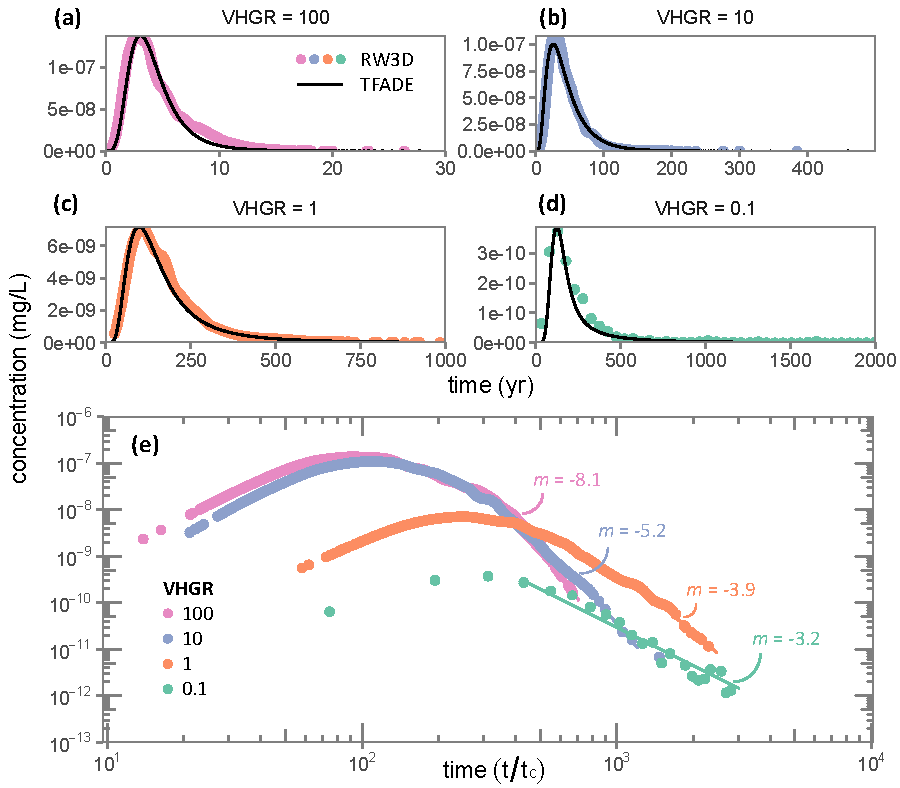
\includegraphics[width=\textwidth]{ch4_figs/tfade.pdf}
	\caption{(a-d) RW3D breakthrough curves (colored points) and fitted TFADE models (black line) measured at the bottom face of the domain (Figure \ref{fig:model}) for the four VHGR scenarios. Note the difference in x-axis travel times. (e) Breakthrough curves are normalized by the characteristic travel time (see SI Appendix Table \ref{ap_c_tc} for details). Measured slopes of tails (denoted as $m$) increase as VHGR decreases, corresponding to increasingly anomalous transport.}
	\label{fig:tfade}
\end{figure}



%
%----------- MSD ---------------%
%
\subsection{Temporal evolution of the plume spatial variance}
\label{ss_3_2}

Temporal evolution of the centered second spatial moments (Equation \ref{eq:msd}) in the longitudinal and transverse directions are superdiffusive and non-Fickian at early times across all VHGR scenarios; late time transitions either remain persistently preasymptotic, or revert to Fickian scaling, depending on the hydraulic gradient conditions (Figure \ref{fig:msd}). We now summarize spreading in the three directions:


\subsubsection{Longitudinal spatial variance}
\label{ss_3_2a}
The magnitude of longitudinal spatial variance (Figure \ref{fig:msd}a) increases with decreasing VHGR, and is preasymptotic and non-Fickian after 32 characteristic times for VHGR = 10, 1, and 0.1. In contrast, when VHGR = 100, late time longitudinal spreading is asymptotic and nearly Fickian ($\phi = $ 0.95 ). Spatial plume variance is around 4 orders of magnitude greater for VHGR = 0.1 compared to VHGR = 100 at all times. This large difference in the scale of spreading results in a wider-ranging residence time distribution between the scenarios (Figure \ref{fig:bottom_yx}a). A strong vertical hydraulic gradient when VHGR = 100 forces particles through nearly all facies in the downward, longitudinal direction (perpendicular to bedding layers), effectively generating an ergodic sample of the system heterogeneity much more rapidly than in scenarios with lower VHGR, thus late time spreading becomes in more Fickian nature. By contrast, at low VHGR, some of the plume remains trapped in fines, and some spreads longitudinally along preferential pathways--both of which stretch the plume.


\subsubsection{Transverse vertical spatial variance}
\label{ss_3_2b}
Like longitudinal spreading, transverse vertical spreading (Figure \ref{fig:msd}b) in VHGR = 100 differs between the other three VHGR scenarios. VHGR = 100 is ballistic (i.e., $\phi >$ 2) at early times ($\phi$ = 2.84) due to entirely advection dominant facies (Table \ref{tab:model_l_k_pe}) and strong lateral connectivity of a high-K incised valley fill (Figure \ref{fig:ivf_xz}a) in the transverse vertical direction that facilitates preferential flow (discussed further in Sections \ref{ss_3_4} and \ref{ss_4_2}). However this spatial variance slows to nearly Fickian spreading ($\phi$ = 0.95) at late times. By contrast, VHGR = 10, 1, and 0.1 are super diffusive at early times (1.77 $\leq \phi \leq$ 1.91) but remain persistently preasymptotic and superdiffusive (1.34 $\leq \phi \leq$ 1.36) at late times rather than reverting to Fickian scaling as in VHGR = 100. 

% F:\Box Sync\Research\Post QE Research\DISSERTATION\02_ade\code/01_msd.R creates msd_time_2amean_ta1.pdf
% which is edited in AI in 02_ade/results/ msd_time_2amean_ta1_ai.pdf
\begin{figure}[ht]
	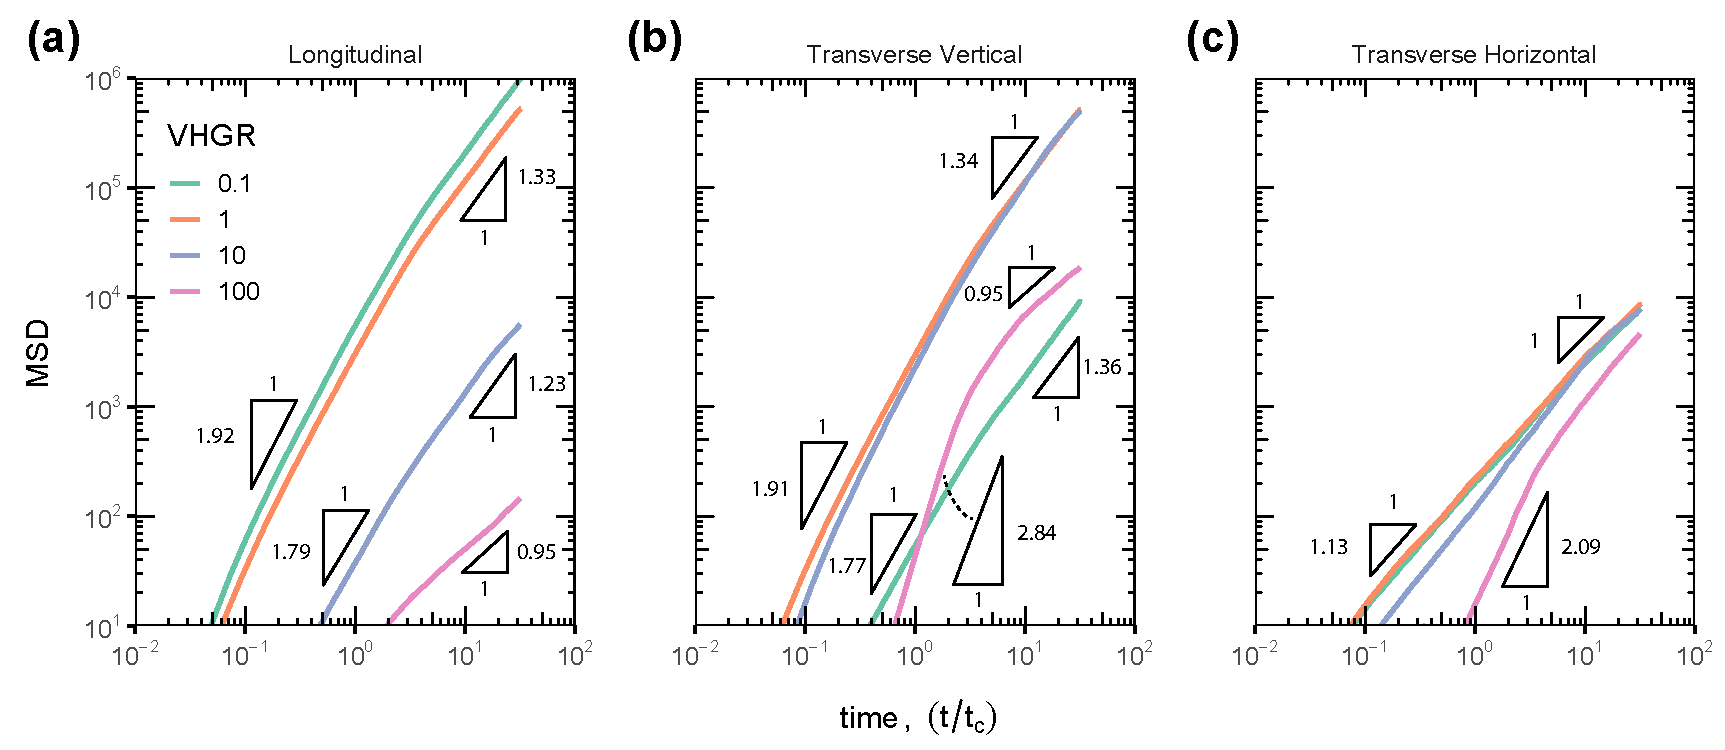
\includegraphics[width=\textwidth]{ch4_figs/msd_time_2amean_ta1_ai.pdf}
	\caption{Temporal evolution of the centered second spatial moments (Equation \ref{eq:msd}) calculated from the distribution of particle trajectories along the (a) longitudinal, (b) transverse vertical, and (c) transverse horizontal directions indicate superdiffusive early time scaling that reduces to less superdiffusive or Fickian scaling in late times, depending on the VHGR and direction of scaling. Triangles at early and late times show the slope of MSD temporal scaling, $\phi$ (Section \ref{ss_msd}).}
	\label{fig:msd}
\end{figure}

The smaller magnitude of transverse vertical spatial variance observed when VHGR = 100 and 0.1 is explained by plume interactions with aquifer heterogeneity. When flow is vertical and downward (VHGR = 100), transverse transport is horizontal, tends to occur along extensive preferential pathways, and is driven toward these pathways by a powerful vertical gradient and all advection dominant facies. When flow is horizontal (VHGR = 0.1), transverse vertical transport is limited by diffusion dominant, laterally extensive paleosols and muds, which prevent spreading along this direction. The middle scenarios (VHGR = 1 and 10) by contrast have stronger vertical gradients to move particles past the first laterally extensive low-K layers, and then a combination of advection, slow advection, and diffusion dominant facies, which creates in greater transverse vertical spreading. 

The smaller magnitude of transverse vertical spatial variance observed when VHGR = 100 and 0.1 compared to VHGR = 10 and 1 is explained by plume interactions with aquifer heterogeneity. When flow is vertical and downward (VHGR = 100), transverse vertical transport occurs along the $y$ direction, which due to relatively high $K'_y$ compared to $K'_z$ should facilitate rapid spreading. However because all facies are advection dominant (Table \ref{tab:model_l_k_pe}) under the influence of powerful vertical gradients, particle trajectories tend to move relatively straight down along non-tortuous particle trajectories. For a different reason, when flow is horizontal (VHGR = 0.1), transverse vertical transport is limited by diffusion dominant, laterally extensive paleosols and muds, which prevent spreading along this direction. The middle scenarios (VHGR = 1 and 10) have a combination of advection, slow advection, and diffusion dominant facies, which simultaneously hold some mass back, and also move particles through laterally extensive low-K facies and layers, all of which results in relatively greater transverse vertical spreading. 


\subsubsection{Transverse horizontal spatial variance}
\label{ss_3_2c}
The absence of a gradient in the transverse horizontal direction (Figure \ref{fig:msd}c) limits superdiffusive early time scaling (1.13 $\leq \phi \leq$ 2.09), and leads to late time asymptotic Fickian scaling ($\phi$ = 1) after 32 characteristic times across all VHGR scenarios. We suspect that transverse horizontal early time superdiffusive scaling when VHGR = 100 is related to the same processes that create early time superdiffusive transverse vertical spreading: migration into preferential pathways. However, since the mean lengths of gravels (and the incised valley fill) in the transverse horizontal $x$ direction are less than in the transverse vertical $y$, the slope of early time superdiffusion is also less.  

In all directions and across all VHGR scenarios tested in this study (except for the VHGR = 100 in the longitudinal direction), superdiffusive early time scaling becomes more Fickian in late times as particles explore more of the system space, and hence the transport is increasingly ergodic. When VHGR = 100, late time longitudinal and transverse second moments approach Fickian scaling (rather than remaining persistently asymptotic), which suggests that an advection dominant system with powerful vertical hydraulic gradients can have a homogenizing impact on the anomalous transport created by system-scale heterogeneity. Furthermore, it illustrates how the degree of non-Fickian effects created when the mean flow direction changes (e.g., persistent superdiffusive scaling) may challenge upscaled approaches that currently fail to capture non-Fickian effects under similar boundary condition transience \citep{guo2020adaptive}.



%
%----------- Influence of preferential flow ---------------%
%
\subsection{Influence of geology on preferential flow and tailing}
\label{ss_3_4}

Non-Fickian transport is influenced by geologic heterogeneity in the hydrofacies model, including a high-K, interconnected incised valley fill, laterally extensive low-K paleosols, and the large volume fraction of low-K mud that plays an important role in diffusion and slow advection dominant transport.

The incised valley fill runs laterally along the $y$ direction, and interconnects to an exit on the down-gradient side of the domain (Figures \ref{fig:ivf_xz}a-b). As VHGR decreases, particles take increasingly horizontal trajectories, and the incised valley fill and other interconnecting sand and gravel lenses act as a conduit for preferential flow that cause more particles exit the down-gradient side of the domain (Figures \ref{fig:ivf_xz}d,f,h,j), where they form clusters around gravel and sand facies (Figure \ref{fig:ivf_xz}b). Across all VHGR scenarios, particle trajectories that exit via the incised valley fill on the down-gradient side tend to exit at earlier timescales compared to other particles that exit the down-gradient side (lighter colored dots in the black oval compared to darker colored dots without outlines in Figures \ref{fig:ivf_xz}c,e,g,i), and compared to particles that take longer flowpaths and exit the bottom of the model at late times (darker colored dots in Figures \ref{fig:bottom_yx}c,e,g,i).


% F:\Box Sync\Research\Post QE Research\DISSERTATION\02_ade\code/
% 03_residence_time_distribution.R creates R objects `p5` and `p6` which are saved as PDFs: rt_t_final_xz_t.pdf, rt_t_final_xz_y.pdf. These are combined with paraview files (front_face_ivf.png and front_face.png) in  C:\Users\rpauloo\Documents\GitHub\kings-river-fan-tprogs\paraview. The generating .pbsm files should also be in that directory.
% finally, these are all combined in 02_ade/results/krf_front_face_ivf.ai
\begin{figure}[H]
  \centering
  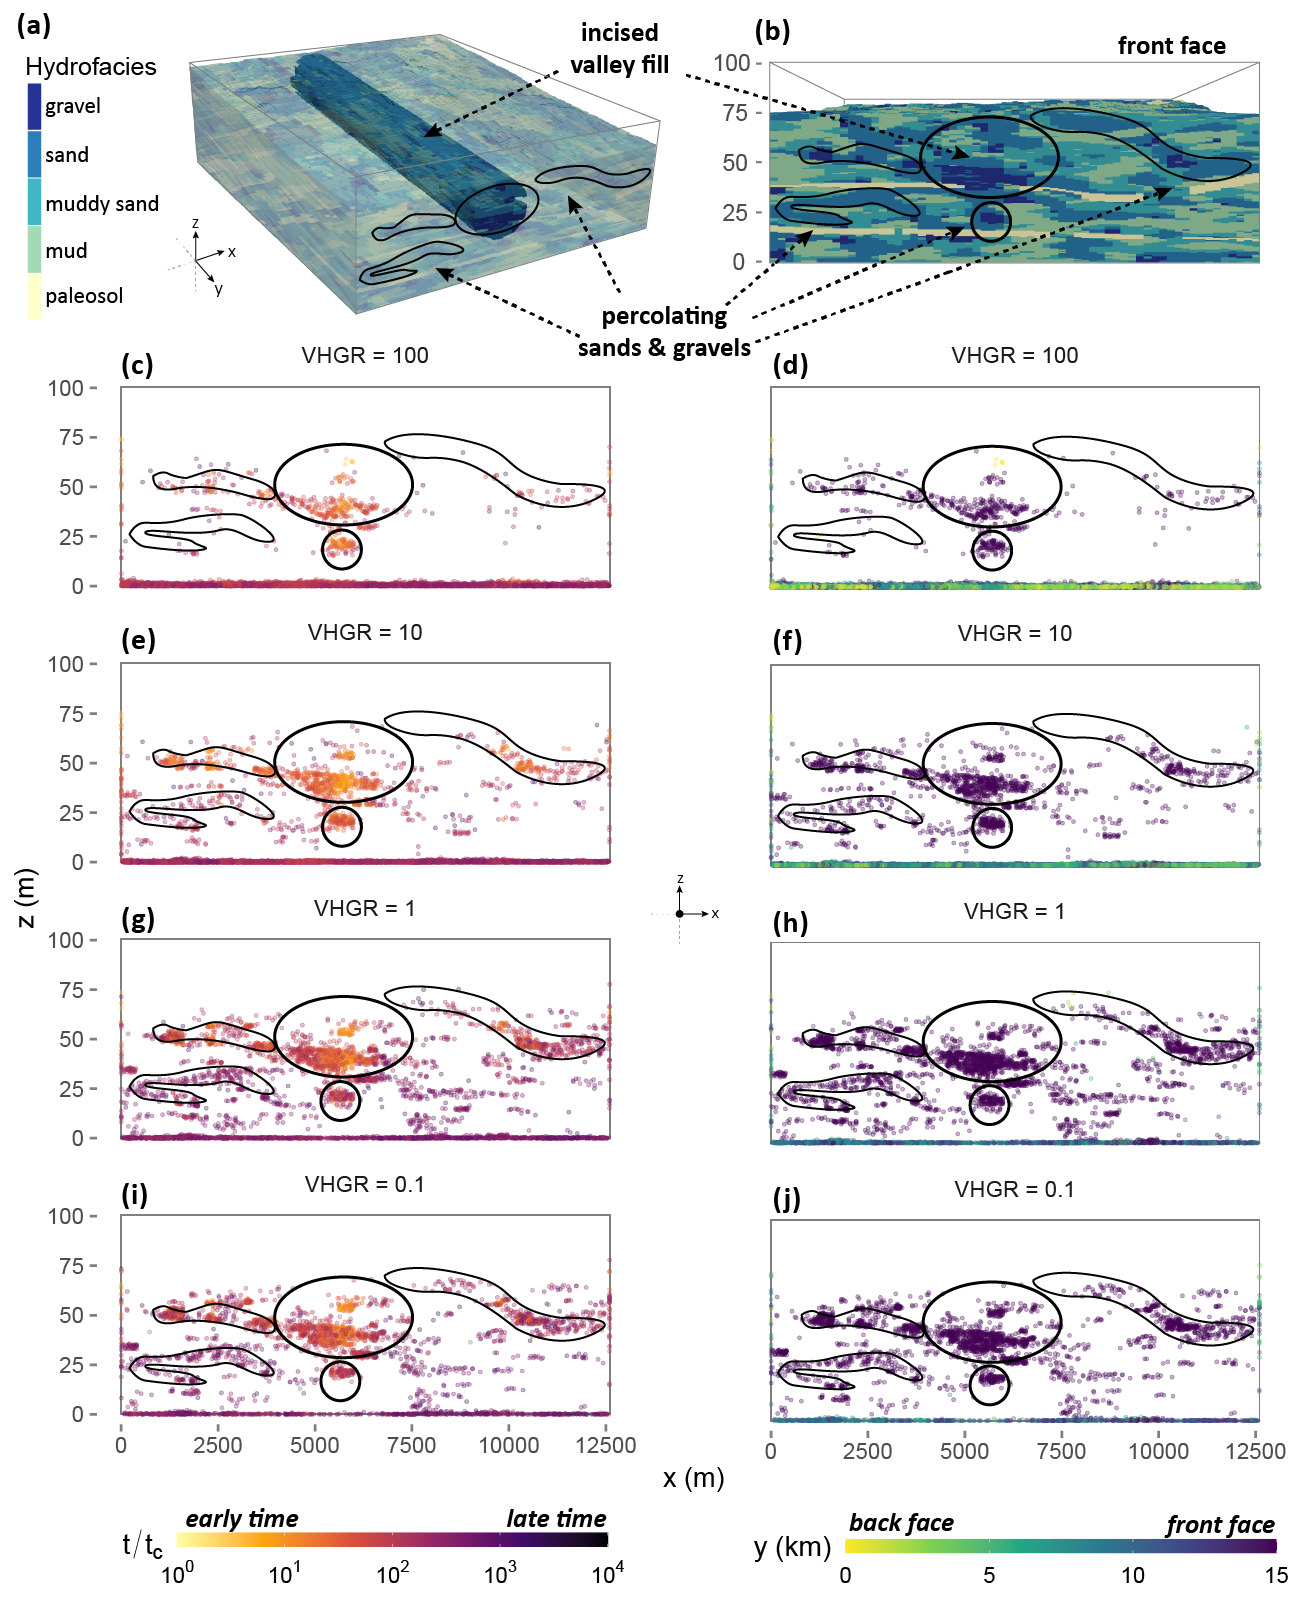
\includegraphics[width=14cm,keepaspectratio]{ch4_figs/krf_front_face_ivf_low_res-01.png}
  \caption{(a) Transparent hydrofacies domain highlighting a lateral, interconnected sand and gravel incised valley fill; (b) The down-gradient side of the domain. A black oval marks the incised valley fill exit, and black outlines mark prominent interconnecting sands and gravel bodies that promote preferential flow. These same regions are marked in black in all other subplots; (c,e,g,i) The final $z$ and $x$ position of particles, colored by the time they exit the domain (residence time); (d,f,h,j) the final $z$ and $x$ position of particles, colored by the length ($y$) into the page, where yellow is the up-gradient side and purple is the down-gradient side. Particle clusters at $z =$ 0 $m$ indicate trajectories that exit the bottom face (Figure \ref{fig:bottom_yx}).}
  \label{fig:ivf_xz}
\end{figure}



% F:\Box Sync\Research\Post QE Research\DISSERTATION\02_ade\code/
% 03_residence_time_distribution.R creates R objects `p`, `p2`, `p3`, and `p4` which are saved as PDFs: rtd.pdf, rtd_inset.pdf rt_t_final_yx_t.pdf, rt_t_final_yx_z.pdf. 
% subplot (b) is made in /paraview/top_face.png and .pvsm
% finally, these are all combined in 02_ade/results/krf_top_face_rtd.ai
\begin{figure}[H]
  \centering
  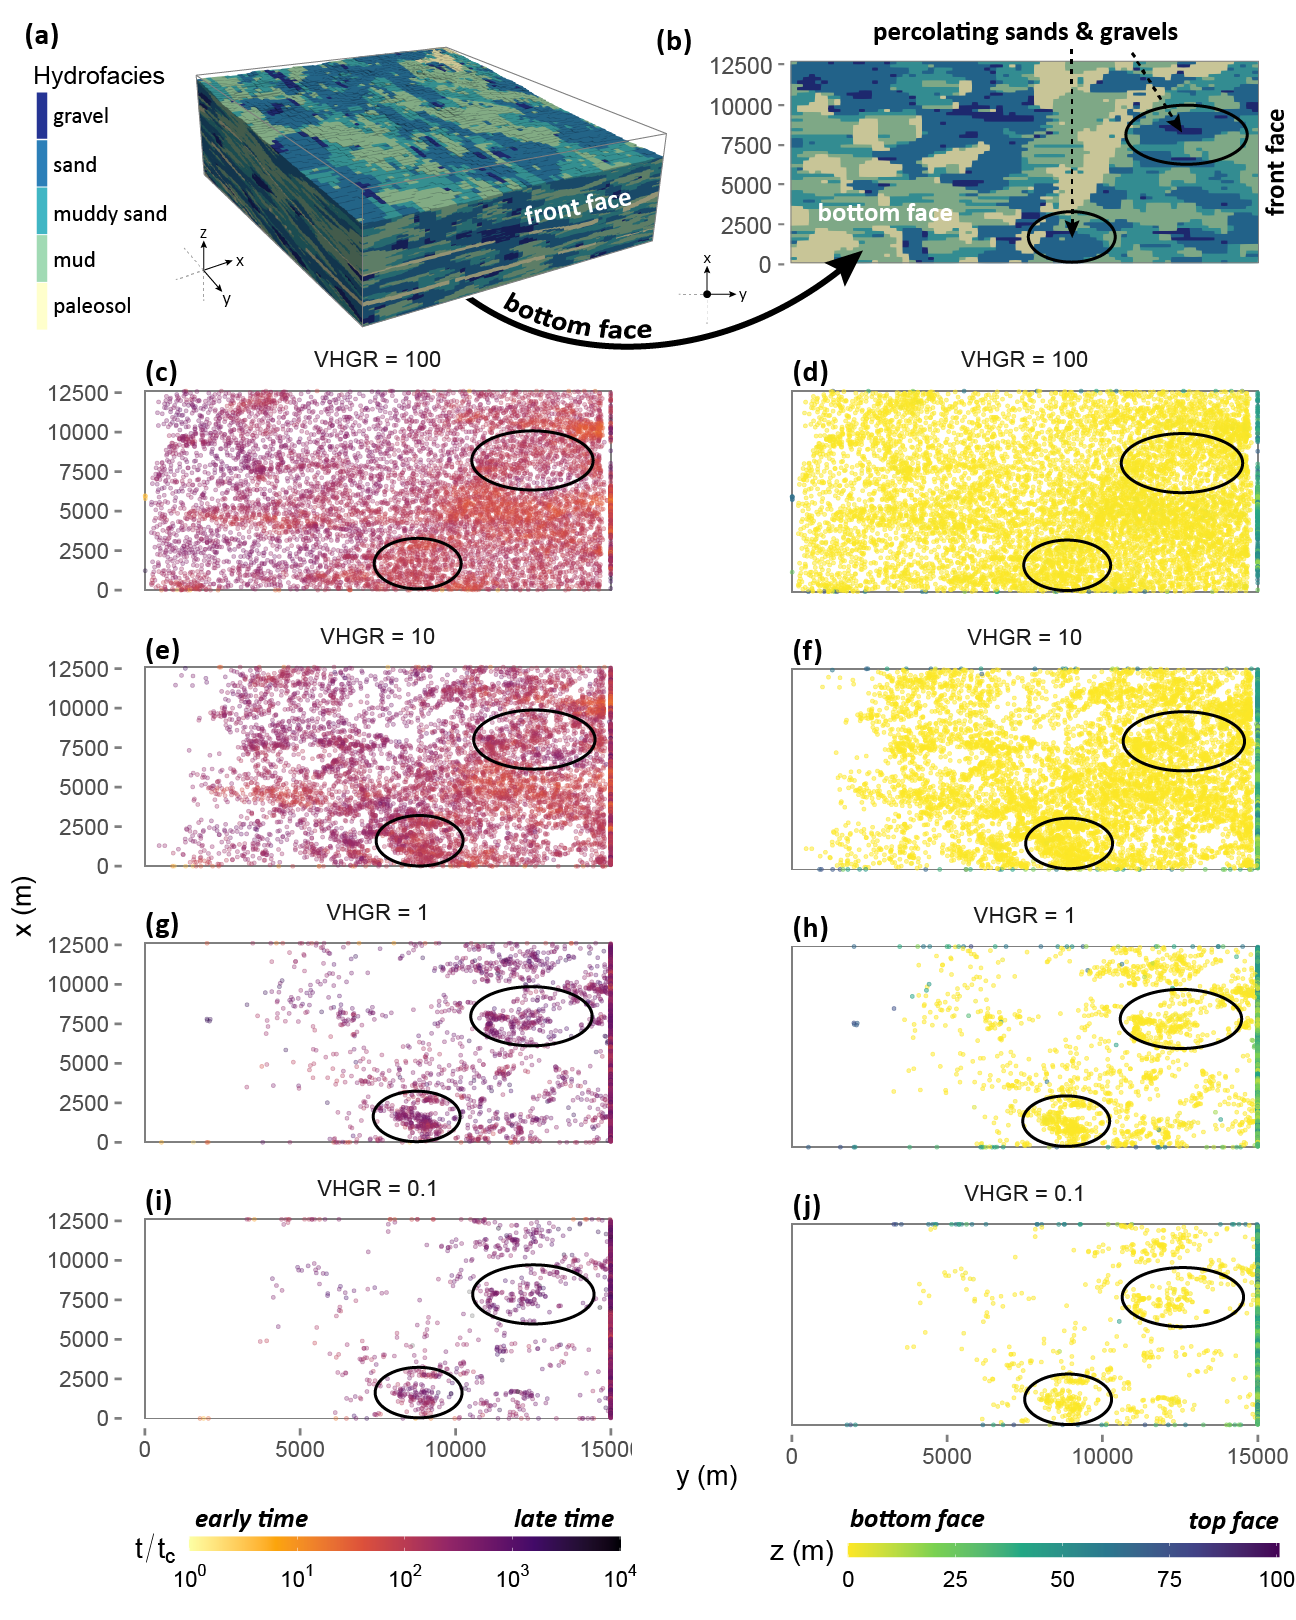
\includegraphics[width=14cm,keepaspectratio]{ch4_figs/krf_top_face_rtd_low_res-01.png}
  \caption{(a) The 3D hydrofacies domain; (b) the bottom of the domain with prominent sand and gravel bodies outlined in black; (c,e,g,i) the final $x$ and $y$ position of particles, colored by the time they exit the domain (residence time); (d,f,h,j) the final $x$ and $y$ position of particles, colored by the length ($z$) into the page, where yellow is the bottom face and purple is the top face. Particle clusters at $y =$ 15 000 $m$ indicate trajectories that exit the down-gradient side of the domain (Figure \ref{fig:ivf_xz}).}
  \label{fig:bottom_yx}
\end{figure}


Notably, even at VHGR = 100 when most particle trajectories take vertical paths and exit the bottom face of the domain (yellow points in Figure \ref{fig:bottom_yx}d), some particles rapidly migrate in the transverse vertical direction along the incised valley fill to exit the down-gradient side (purple dots in the black oval in Figure \ref{fig:ivf_xz}d). Moreover, early time arrival through the incised valley fill when VHGR = 100 (Figure \ref{fig:ivf_xz}c) suggests that transverse horizontal preferential flow still occurs along interconnected coarse facies even under strong vertical gradients, and explains the ballistic early time transverse vertical scaling ($\phi = $ 2.84) in this scenario (Figure \ref{fig:msd}b).

Laterally extensive low-K paleosols limit (Figure \ref{fig:ivf_xz}b) the vertical migration of particles, and create segmented breakthrough along the down-gradient side of the domain where particles tend to exit above or below paleosol layers, but rarely through them (Figures \ref{fig:ivf_xz}d,f,h,j).




%--------------------------------------------------------%
%	DISCUSSION
%--------------------------------------------------------%

\section{Discussion}

%
%----------- hydraulics ---------------%
%
\subsection{Mean flow direction modulates the degree of non-Fickian transport}
\label{ss_4_1}

In clastic sedimentary environments, significant regional-scale vertical anisotropy in K caused by stratification of facies and seasonal pumping and recharge can create strong vertical hydraulic gradients that in turn cause oscillations in mean flow direction. This study aimed to assess impacts of these shifting flow directions on the regional-scale, non-Fickian transport of nonpoint source contaminants in a typical alluvial aquifer-aquitard complex. Results demonstrate that shifting VHGR can \textit{modify the degree} of non-Fickian transport. Decreasing VHGR led to increasingly non-Fickian transport, measured by tailing at a control plane along the bottom face of the model, increased and persistent non-Fickian scaling of the second spatial moment, and increased preferential flow along interconnected high-K facies. 

Our results are consistent with previous studies which demonstrate that non-Fickian spreading measured (at a target well) can accompany the change from plume migration along an ambient groundwater gradient, to transient pump-and-treat conditions \citep{labolle2001role, guo2019upscaling, guswa2000slow}, which facilitates the release of mass stored in fine-grained material. Results illustrate that non-Fickian spreading of a nonpoint source plume depends on the mean flow direction, modified in many aquifer systems worldwide by ubiquitous pumping wells \citep{Famiglietti2014, Gleeson2012, wada2010global} that increase vertical head gradients and drive flow downward. 

Together, the increasingly non-Fickian effects (e.g., increased tailing, greater spatial spreading) that result as the mean flow direction shifts from horizontal to vertical suggest a conceptual model of nonpoint source transport in agriculturally intensive alluvial groundwater basins characterized by oscillating patterns of more Fickian vertical migration during periods of intense pumping and recharge, interspersed by periods of persistently non-Fickian lateral plume stretching under ambient groundwater flow when pumps are off and fields are not irrigated, except perhaps in areas with significant natural vertical anisotropy in K. These insights into the dependence of non-Fickian transport on mean flow direction bear importantly on efforts to model and manage nonpoint source contamination like salts \citep{hansen2018quantifying} and nitrates \citep{pasten2014assessment} in large irrigated basins where the flow boundary conditions (and hence VHGR) are inherently transient. Thus, an unresolved challenge for existing methods that upscale the advection-dispersion equation \citep{neuman2009perspective} is the ability to capture the varying non-Fickian behavior of regional, nonpoint source transport resulting from changes in the mean flow direction \citep{guo2020adaptive}. This study advances a hydrogeologic perspective towards understanding the physical genesis of this challenge.

%We emphasize that non-Fickian transport is driven by the interaction of hydraulics with well-characterized geologic heterogeneity. VHGR controls the ratio of advective to diffusive flux in hydrofacies (i.e., the Peclet number), and the mean flow direction, and hence the anisotropy encountered (i.e., flow parallel, perpendicular, or oblique to layers). Furthermore, results indicate that multiple scales of geologic heterogeneity (e.g., laterally extensive paleosols, a highly conductive incised valley fill) clearly influence plume-level non-Fickian transport, and hence, better characterization of multi-scale geology is imperative to modeling regional-scale transport \citep{zhang2006nonpoint}.



%
%----------- geology ---------------%
%
\subsection{Hydrogeologic heterogeneity underpins non-Fickian transport}
\label{ss_4_2}

Differing degrees of non-Fickian transport and plume spreading arise from hydrogeologic heterogeneity in the study site, which can be understood in terms of high ln-K variance, the transition from diffusion to advection dominant transport, and persistently non-Fickian transport caused by preferential flow and mass holdback.

%
%----------- ln K variance ---------------%
\subsubsection{The role of high ln-K variance}
\label{ss_4_2_1}

The geologically-based conductivity field in this study represents multi-scale heterogeneity, by which we mean multiple geologic sequences with large variance in K \citep{weissmann1999multi}, in contrast to stochastic Gaussian models with typical ln-K variances, $\sigma^2_{lnK} < $ 1 or 2 \citep{gelhar1993stochastic, rubin2003applied}. For our study site, $\sigma^2_{lnK} = $ 8.3, approximated by $\sigma^2_{lnK} \approx R^2/3$ \citep{fogg2016debates}, where $R$ is the range between the minimum and maximum values of K in orders of base 10 magnitude (i.e., 5 in this study).  Results suggest that non-Fickian transport is strongly affected by the transition of low-K facies along diffusion, slow advection, and advection dominated system states (Section \ref{ss_4_2_2}); and by the presence of an incised valley fill and laterally extensive, low-K paleosols (Section \ref{ss_4_2_3}). Furthermore, the persistently preasymptotic MSD scaling observed in some VHGR scenarios reinforce the notion suggested by other researchers \citep[e.g.][]{matheron1980transport, neuman1990universal, zhang2007persistence} that the late-time transition from non-Fickian to Fickian transport may never occur in natural geologic formations under certain gradient conditions. Thus, a key component to capturing non-Fickian effects is proper parameterization of the ln-K variance of the spatial heterogeneity.

%
%----------- Pe ---------------%
\subsubsection{Transitions between diffusion and advection dominant transport}
\label{ss_4_2_2}
In a spatial model with ln-K variance, transience in the hydraulic gradients can create systems that range from fully advection dominant, to systems of mixed advection and diffusion dominance, the latter of which will have greater non-Fickian effects.

As VHGR increases and flow is increasingly vertical, the hydrofacies Peclet number (Table \ref{tab:model_l_k_pe}) and hence advection dominant transport also increases. Importantly, in our study site, as VHGR increases from 0.1 to 100, the mud and paleosol facies shift from diffusion dominant ($P_e < $ 1) to slow advection and advection dominant ($P_e > $ 1). Consequently, high VHGR causes mass to migrate nearly straight through fines, consistent with the findings of \citet{guswa2000slow}, who observed accelerated solute release from low permeability zones under the influence of pumping in a slow-advection mass transfer system. In contrast to a diffusion dominant system, pumping would have little to no effect on the mass release from fines. Slow-advection is thus more related to the groundwater velocity, as opposed to a mass transfer model that strictly assumes diffusive controls on mass release from low permeability lenses. In this study, the decrease in non-Fickian transport observed at increasing VHGR and hence $P_e$ leads us to speculate that hydraulic forcings may exert a similar effect on transport as aquifer-aquitard spatial properties \citep[e.g.][]{zhang2006nonpoint, zhang2007predicting, yin2020super, zhang2013impact}. For instance, \citet{zhang2013impact} found that in domains containing hydrofacies with relatively short mean lengths, particles moved more rapidly between hydrofacies, which increased the likelihood for solutes to sample the full range of flow velocities, and thus more rapidly reach ergodicity. Similarly, we find that strong vertical flow (e.g., VHGR = 100) can push particles through all facies alike, thus accelerating mass transport between hydrofacies and rapidly reaching ergodicity. Furthermore, \citet{zhang2007predicting, zhang2013impact} observed that diffusion limited vertical floodplain layer thicknesses controlled late time non-Fickian solute tailing. Similarly, our results suggest that higher VHGR can shift facies from diffusion to advection dominance and diminish non-Fickian tailing. Hence, non-Fickian transport imparted by spatial heterogeneity should not be viewed as constant, but rather, as continually modified by hydraulic transience.

%
%----------- preferential flow and massholdback ---------------%
\subsubsection{Persistent non-Fickian transport}
\label{ss_4_2_3}

Describing persistent, late time, non-Fickian transport observed in this study (Section \ref{ss_3_2}) remains a modeling challenge. We now discuss the factors that control persistently preasymptotic non-Fickian transport, specifically how it relates to hydrofacies heterogeneity, preferential flow, and the transition from diffusion to advection dominant transport.

First, the super-linear growth of early time plume spatial variance observed in this study (i.e., superdiffusion, $\phi > $ 1) is consistent with other simulations in heterogeneous porous media \citep{zhang2013impact, kang2014pore, hunt2011dispersion}. The conventional understanding of this phenomenon is that preferential flow in highly permeable facies stretches the plume front downstream, while the trailing plume tail remains trapped by low-permeability facies near the source \citep{fiori2003flow, dagan2003flow, zhang2014linking, labolle2001role}. As ergodicity is reached in late times, plume spatial variance approaches Fickian scaling, which has been observed in numerous experiments \citep[e.g.][]{kang2014pore, le2010non, cortis2004numerical} and is relatively easier to model. However, persistently asymptotic behavior may never arise because the time needed to reach asymptotic behavior in natural geologic systems may be sufficiently large that the solute will encounter new spatial nonstationarities along the displacement distance before Fickian scaling is reached, and is thus always in a state of transition, never reaching asymptotic behavior \citep{matheron1980transport, gillham1984advection, neuman1990universal}.

We speculate that the multiple-scale geologic heterogeneity in our study area causes persistently non-Fickian superdiffusion at late times in longitudinal and transverse directions for all VHGR $\leq$ 10. This persistent late time non-Fickian transport is supported by \citet{labolle2001role}, who noted persistent preasymptotic ambient transport in a similar well-connected, hydrofacies-based alluvial fan model. Moreover, \citet{zhang2007persistence} found that transition times in simple, 2D uniform media were so large, that the authors speculated that in natural geologic media with multiple‐scale heterogeneity, the transition from anomalous to Fickian transport may never complete. Complimentary to these observations, our results indicate that sufficiently high VHGR can reduce the impact of mass sequestration in fines, lead to a more compact plume in all directions, and hence, promote asymptotic late time Fickian scaling in all dimensions, thus lending itself towards being more appropriately described by an upscaled model.  

The important role of preferential flow on persistent non-Fickian transport is illustrated by the impact of a lateral, connected, incised valley fill and other prominent interconnecting sand and gravel bodies (Figure \ref{fig:ivf_xz}a). When VHGR = 100, rapid particle migration into the incised valley fill transverse vertical to the mean flow direction resulted in early time hyper-ballistic scaling ($\phi = $ 2.84) of transverse vertical MSD that slowed to nearly Fickian scaling ($\phi = $ 0.95) at late times as ergodicity was reached. In contrast, when VHGR = 10, 1, and 0.1, preferential flow along high-K networks stretched some of the plume at the same time that fines sequestered other parts of it, leading to persistent and oftentimes a greater magnitude of late-time spreading ($\phi = $ 1.34 - 1.36). Across all scenarios, particles traveled laterally through the incised valley and exited the down-gradient side at relatively earlier times (Figure \ref{fig:ivf_xz}c). Observations of faster transport along highly-permeable, interconnected sand and gravel lenses are consistent with numerous studies of preferential flow \citep{winograd1976major, jussel1994transport, moreno1994flow, tsang1998flow, fogg1986groundwater, heeren2010preferential, maxwell2008contamination, zheng2003analysis, weissmann2004influence, labolle2001role}. 

Final particle positions and the hydrofacies they occupy at that time further illustrate the importance of advection and diffusion dominant transport and preferential flow. When VHGR = 100 and advection dominates transport, particles are nearly indiscriminate in terms of the facies they occupy upon exiting the bottom face of the domain (i.e., even spatial distribution of yellow dots in Figure \ref{fig:bottom_yx}d). By contrast, when VHGR = 0.1, spatial patterns of particles that exit the bottom face of the domain (yellow dots in Figure \ref{fig:bottom_yx}j)) and the down-gradient side (purple dots in Figure \ref{fig:ivf_xz}j) correlate with more conductive, high K facies (blue and dark blue sand and gravel in Figures \ref{fig:bottom_yx}b and \ref{fig:ivf_xz}b). This indicates preferential flow along interconnecting sand and gravel lenses, and partly explains the increased non-Fickian transport with decreasing VHGR as a result of relatively rapid plume stretching along these fast flowpaths. 

%Surprisingly, VHGR = 0.1 and 100 exhibit a more similar magnitude of transverse vertical MSD, even though the mean flow directions in these scenarios were the most extreme tested in this study, ranging from mostly horizontal to mostly vertical. However, this seemingly counter-intuitive finding can be reconciled by considering the interaction of mean flow direction, the spatial heterogeneity of the domain, and the role of advection and diffusion dominant hydrofacies on transport. When VHGR = 100, particle trajectories move nearly straight down (Figure \ref{fig:res_time_dist_yx}d), even migrating through laterally extensive low-K hydrofacies, which under the influence of strong gradients become advection dominant (Table \ref{tab:model_l_k_pe}), thus helping to facilitate this vertical transport. 
%The temporal evolution of the hydrofacies proportions support these observations, and show higher paleosol occupancy for high VHGR, and advection-driven mass transfer out of paleosols (Figure \ref{fig:phft}). 
%For a different reason, we observe similar scaling of the transverse vertical MSD when VHGR = 0.1. In this case, flow is more horizontal and parallel to the bedding layers, but the transverse vertical mass transfer is limited by abundant, laterally extensive, and muds and paleosols which are diffusion dominant at these hydraulic gradients (Table \ref{tab:model_l_k_pe}), which prevents mixing along the transverse vertical direction, and thus limits the magnitude of transverse vertical MSD scaling. By contrast, plumes in the intermediate scenarios (VHGR = 1 and 10) exhibit a greater magnitude of transverse vertical spreading. In these scenarios, vertical hydraulic gradients are sufficiently large enough to drive vertical transport, and the mud and paleosol hydrofacies can be advection dominant, which increases transverse mass exchange along these facies, and thus the plume spreads more in the transverse vertical direction.



%
%----------- upscaled models ---------------%
%
\subsection{Implications for upscaled transport models}
\label{ss_4_3}

The varying degrees of non-Fickian transport that arise from the interaction of hydraulics and geologic heterogeneity challenge the application of the advection-dispersion equation towards subsurface transport problems in natural geologic media. At regional scales (e.g., tens to hundreds of kilometers), subsurface characterization may be intractable or cost-prohibitive, and even if reliable subsurface models were available, the computational complexity of solving transport over these scales would be enormous. Hence, regional upscaled transport models are needed. These upscaled models must be able to represent non-Fickian effects created by preferential flow in connected high‐conductivity facies, mass transfer processes between high‐ and low‐conductivity media, and as we show in this study, the different degrees of non-Fickian transport introduced by changes in the mean flow direction due to varying VHGR (e.g., in the case of significant pumping and recharge).

In a previous study, \citet{guo2020adaptive} demonstrated an adaptive multirate mass transfer (aMMT) model which improved breakthrough curve estimation for diffusion dominant transient flow by incorporating time-dependent mass transfer coefficients based on the equivalent flow velocity. However, the aMMT approach failed to capture tailing in breakthrough curves when the mean flow direction changed, as in the case of shifting VHGR. In this study, we extend the work of \citet{guo2020adaptive} and illustrate that as VHGR changes, the transition from diffusion to slow advection and advection dominance in the discrete hydrofacies of a system can fundamentally change the mass transfer processes. Specifically, high VHGR (provided it creates system-wide advection dominance) can cause solutes to move nearly straight through facies (e.g., Figures \ref{fig:model} \ref{fig:bottom_yx}d even though the vertical effective K is much less than the horizontal effective K, whereas low VHGR (diffusion to slow advection dominance some facies) can lead to mass holdback in fines (Figure \ref{fig:tfade}) and strong preferential flow (Figures \ref{fig:ivf_xz}h,j and \ref{fig:bottom_yx}h,j). Thus, a future promising direction towards the goal of improving estimation of late time tailing under transient flow is to quantify changes in VHGR, $P_e$, mean flow direction, and characteristic length scales along the mean flow direction, and relate these to mass transfer processes parameters in a upscaled model (e.g., aMMT).




%
%----------- limitations ---------------%
%
\subsection{Study limitations and additional considerations}
\label{ss_limitations}

We explore highly detailed nonpoint source plume evolution across a series of steady state flow simulations in order to observe regional-scale, long term transport under conditions that represent the transition from relatively ambient groundwater flow to predominantly vertical flow. However, these steady state simulations do not the capture mass transfer effects that occur when hydraulic boundary conditions rapidly change, as in the case of a pumping well being turned on. For example, \citet{bastani2020effects} found that transport models based on steady state flow did not capture short-term oscillations of nitrate concentrations in pumping wells at the local scale. Similarly \citet{guo2020adaptive} showed that the aMMT model failed to reproduce transport when the flow direction changed, and \citep{labolle2001role} observed the release of mass stored in fine-grained material when boundary conditions changed from plume migration along an ambient groundwater gradient, to transient pump-and-treat conditions. Thus a future challenge is to explore nonpoint source plume evolution in a transient simulation that incorporates transitions between each VHGR scenario, and which represents the hydraulic conditions observed in natural irrigated basins with extensive pumping. 

Heterogeneous porous media affects reactive solute transport by controlling solute mixing and residence times \citep{perez2019organic}, which may be more important for certain solutes and depth zones. In this study, we simulate a nonreactive solute, which may not be suitable for some nonpoint source contaminants in fully saturated groundwater. More research needed on how reaction rates may alter the non-Fickian effects explored in this study, for instance, by mineral dissolution of the domain which adds a source term \citep{schoups2005sustainability}, or in the case of nitrates, by denitrification in the soil zone \citep{lee2006nitrogen}. 

It is well known that hydrofacies geometry influences contaminant transport, and hence, our study is best interpreted with respect to the characteristic geology of the domain. For example, \citet{yin2020super} found that larger hydrofacies width increased high-permeability connectivity, and thus superdiffusion; conversely, larger mean hydrofacies thickness slowed solute migration and reduced plume scaling. Any extrapolation the results presented herein to other areas should be accompanied by a careful consideration of the hydrogeology of the new study site.



%--------------------------------------------------------%
%	CONCLUSIONS
%--------------------------------------------------------%
\section{Conclusions}
\label{s_5}


We simulated 3D steady state groundwater flow and nonpoint source contaminant transport in a regional scale (15 $km$ x 12.6 $km$ x 100 $m$) geostatistical representation of a heterogeneous alluvial aquifer-aquitard system. In horizontally stratified clastic sedimentary aquifer systems it is common for the strong vertical anisotropy of hydraulic conductivity to produce spatially and temporally varying vertical and horizontal components of the hydraulic gradient, in turn producing a complex interplay between the stratified heterogeneity and physical transport processes. These effects can be augmented and made highly transient by the effects of pumping and recharge in, for example an agricultural system where oscillations between primarily horizontal and primarily vertical flow are caused by seasonal fluctuations in pumping as well as the recharge produced by irrigation. Thus we tested the impact of these varying mean flow directions on non-Fickian transport, and observed increasingly non-Fickian transport as flow was increasingly horizontal (i.e., when the VHGR decreased). Importantly, when VHGR was large (e.g., 100), the plume was more compact: particle trajectories exhibited late time asymptotic Fickian scaling of spatial variance, and moved perpendicular to the direction of aquifer bedding (even though the vertical effective K is much less than the horizontal effective K), and nearly straight through high- and low-conductivity facies alike. As VHGR decreased (e.g., 10 and 1) flow became more horizontal and transport was more non-Fickian -- particle trajectories increasingly moved along laterally extensive facies, took preferential flowpaths, and exhibited greater (and preasymptotic) spatial spreading and tailing in breakthrough measured along a control plane at the bottom face of the model. Hence, the non-Fickian transport imparted by spatial heterogeneity should not be viewed as constant, but rather, as continually modified by hydraulic transience that may transition facies from diffusion to advection dominance and thus alter non-Fickian mass transfer dynamics. These results illustrate why conventional methods to upscale anomalous transport under transient flow conditions remains a challenge, and indicates that future efforts to upscale regional-scale, transient nonpoint source transport may benefit by incorporating information on the time-dependent changes in VHGR, $P_e$, mean flow direction, and characteristic length scales along the direction of mean flow.


\clearpage
